\subsection{Preliminary Analysis}
\begin{figure}[h]
	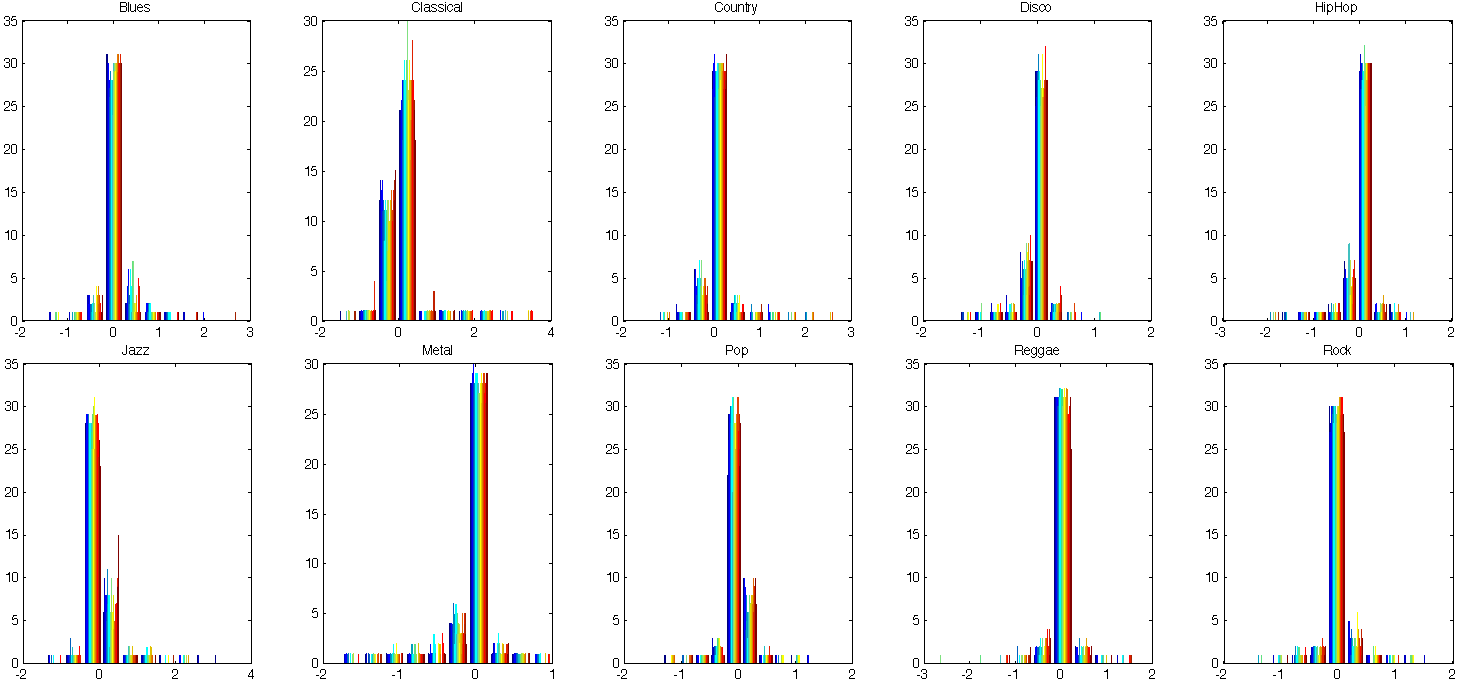
\includegraphics[width=\textwidth]{histgram_mfcc.png}
	\caption{Plots for time-averaged means of MFC coefficients for the 10 genres, every colored line represents one song}
\end{figure}
We see that the distribution of the means of MFC coefficients do indeed differ across genres, suggesting that MFCC is an informative feature for classification.

\begin{figure}[h]
	\begin{subfigure}[b]{0.49\textwidth}
		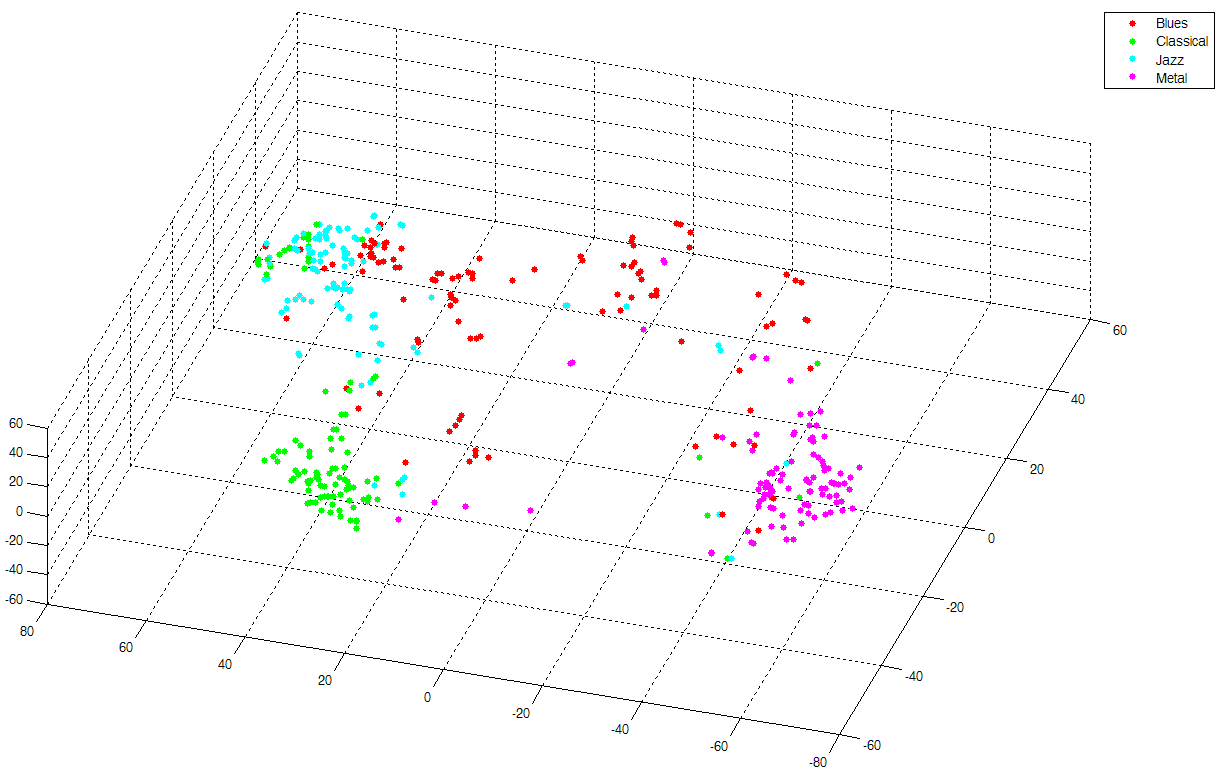
\includegraphics[width=\textwidth]{blues_classical_jazz_metal.png}
		\caption{t-sne subplots for Blues, Classical, Jazz, Metal showing clean separability}
		\label{fig:tsne1}
	\end{subfigure}
	\hfill
	\begin{subfigure}[b]{0.49\textwidth}
		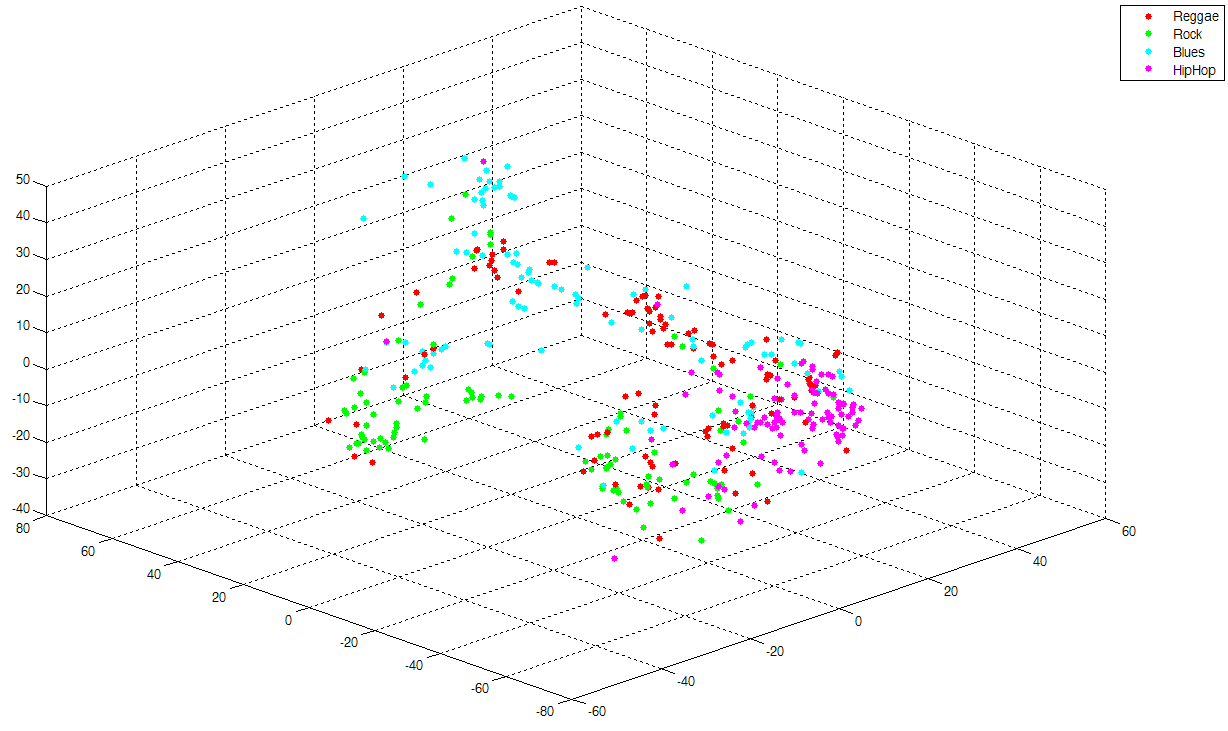
\includegraphics[width=\textwidth]{reggae_rock_blues_hiphop.png}
		\caption{same t-sne subplots for Reggae, Rock, Blues, Hip-Hop showing confusion}
		\label{fig:tsne2}
	\end{subfigure}
	\caption{t-sne plots in 3-D of a projection of 960-dimensional MFCC FV}
\end{figure}
We also see even in an extremely compressed 3-dimensional projection of the MFC data, t-sne is able to discern clear clusters of songs in each genre. This gives us a hint as to which genres are easily separated and which are easily confused.
\subsection{Combinations of features with different classifiers}
\begin{figure}[H]
	\begin{tabular}{|l|l|l|l|l|l|l|l|l|}
		\hline
					& 1.KNN3  & 2,KNN5  & 3.SVM-Lin & 4.SVM-RBF & 5.GNB  & 6.RF  & Softvote 2,3,5,6  & Hardvote 2,3,5 \\ \hline
		Min error   & 0.343 & 0.333 & 0.255  & 0.384  & 0.37 & 0.288  & 0.245  & 0.261 \\ \hline
		Feature set & \multicolumn{3}{l|}{\begin{tabular}[c]{@{}l@{}}MFCC\\ HCDF\end{tabular}} & MFCC    & \begin{tabular}[c]{@{}l@{}}MFCC\\ energy\end{tabular} & \begin{tabular}[c]{@{}l@{}}chroma\\ HCDF\end{tabular} & \begin{tabular}[c]{@{}l@{}}MFCC\\ chroma\\ brightness\end{tabular} & \begin{tabular}[c]{@{}l@{}}HCDF\\ brightness\end{tabular} \\ \hline
	\end{tabular}
	\caption{10-fold CV classification error rate for different classifiers and the features that performed the best, for full data table see figure \ref{fig:all_results}}
	\label{fig:classifiers}
\end{figure}
We see in figure \ref{fig:classifiers} that the feature set of MFCC, chroma and brightness performed with 0.245 error rate with a soft voting algorithm of KNN5, SVM(Linear kernel) Gaussian NB, and Random Forest.
\subsection{Fisher vectors vs PCA of raw timeframe data}
\begin{figure}[h]
	\floatbox[{\capbeside\thisfloatsetup{capbesideposition={right,top},capbesidewidth=4cm}}]{figure}[\FBwidth]
	{\caption{The error rates of two Feature FV against their raw data counterparts with two classifiers}\label{rawdata}}
	{
	\begin{tabular}{|l|l|l|}
		\hline
		& KNN3  & SVM-Lin \\ \hline
		MFCC FV         & 0.343 & 0.255   \\ \hline
		MFCC Raw data   & 0.461 & 0.396   \\ \hline
		Chroma FV       & 0.605 & 0.558   \\ \hline
		Chroma Raw data & 0.671 & 0.679   \\ \hline
	\end{tabular}
	}
\end{figure}
In figure \ref{rawdata} we see that the generated Fisher Vectors performs better than just a simple collection of raw data vectors
